\documentclass[10pt]{beamer}
%\documentclass[handout]{beamer}
%\usepackage{pgfpages}
%\pgfpagesuselayout{2 on 1}[a4paper,border shrink=5mm]

\mode<beamer>{
	\usetheme[hideothersubsections,right,width=22mm]{Goettingen}
}

\title{Thesis Defense}
\subtitle{Electrochemical Biosensor Array Characterization}
\author[M.W. Jibson]{Matthew W. Jibson}
\institute{Colorado State University}
\titlegraphic{
\includegraphics[width=20mm]{figures/biosensorchip-black.png}}
\date{29 May 2009}

\begin{document}

\setbeamertemplate{footline}[page number]
\setbeamertemplate{bibliography item}[text]

\begin{frame}
	\titlepage
\end{frame}

\section{Introduction}
\subsection{Neurotransmitter Detection}
\begin{frame}{Neurotransmitter Detection}
	\begin{itemize}
		\item need to detect neurotransmitters, like nitric oxide (NO)
		\item need to detect how much NO there is at many places at once, so we need a gradient
		\item until recently, sensors have been larger than cells, so not possible
		\item microelectrodes are now around $100 \mu \mathrm{m}$ to $1 \mu \mathrm{m}$
		\item discrete sensors will not work: too bulky
		\item integrated sensors save the day
		\item small feature size: on-chip array of sensors and potentiostats
	\end{itemize}
\end{frame}

\subsection{Objectives}
\begin{frame}{Objectives}
	\begin{itemize}
		\item Anita Karegar designed a chip 2 years ago with an array of sensors
		\item first ever design with hypotheses about shape, size, distance and configuration of electrodes
		\item this thesis reviews those design hypotheses, tests them, and finds some conclusions
		\item also, we test some living mouse-ovary slices
	\end{itemize}
\end{frame}

\section{Background and Existing Approaches}
\subsection{Introduction to Electrochemistry}
\begin{frame}{Introduction to Electrochemistry}
	\begin{itemize}
		\item used to determine compounds in a solution: how much of what
		\item put electrodes in a solution
		\item apply a potential difference across them
		\item if it is high/low enough, electrons will move over (reduction, oxidation)
		\item force potential to not change, thus current flows
	\end{itemize}
\end{frame}

\begin{frame}{Amperometry}
	\begin{itemize}
		\item constant potential
		\item measure current spikes from injected or diffused compounds
		\item good for real-time measurements
		\item bad at detecting multiple compounds
	\end{itemize}
	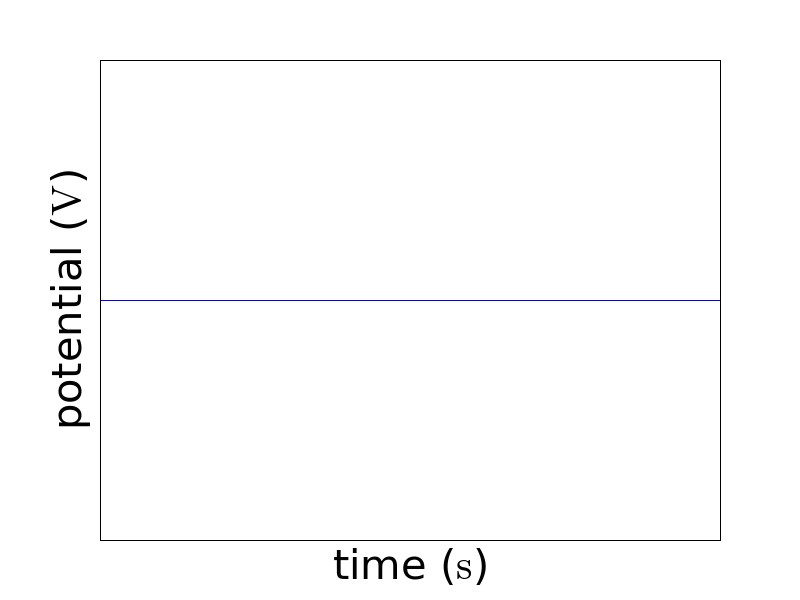
\includegraphics[width=0.5\linewidth]{figures/amperometry.png}
	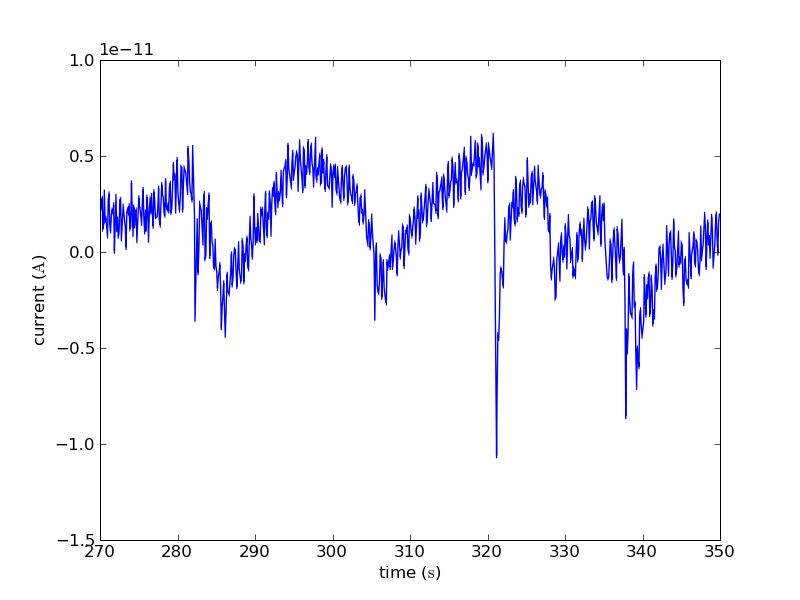
\includegraphics[width=0.5\linewidth]{figures/216.png}
\end{frame}

\begin{frame}{Cyclic Voltammetry}
	\begin{itemize}
		\item potential changes linearly with time up and down
		\item compounds have a specific potential at which they reduce/oxidize
		\item good for multiple compound detection
		\item bad at real-time detection
	\end{itemize}
	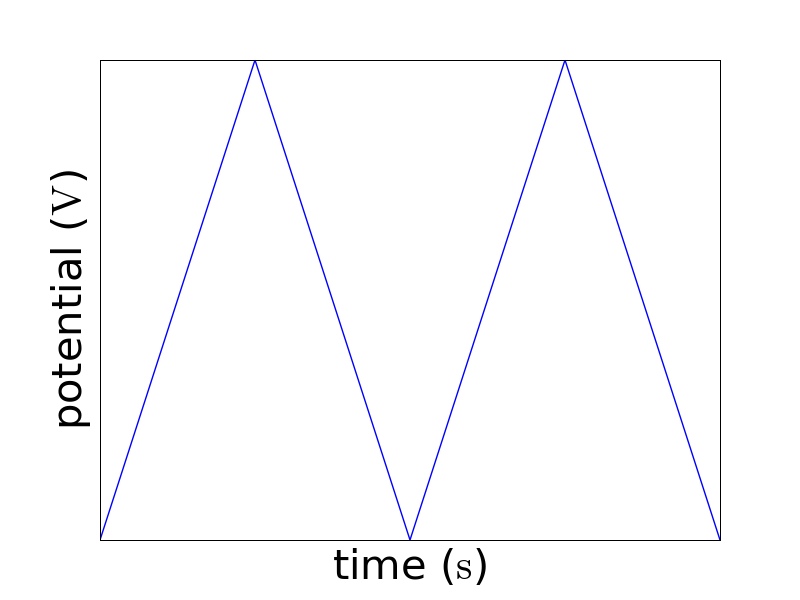
\includegraphics[width=0.5\linewidth]{figures/cv.png}
	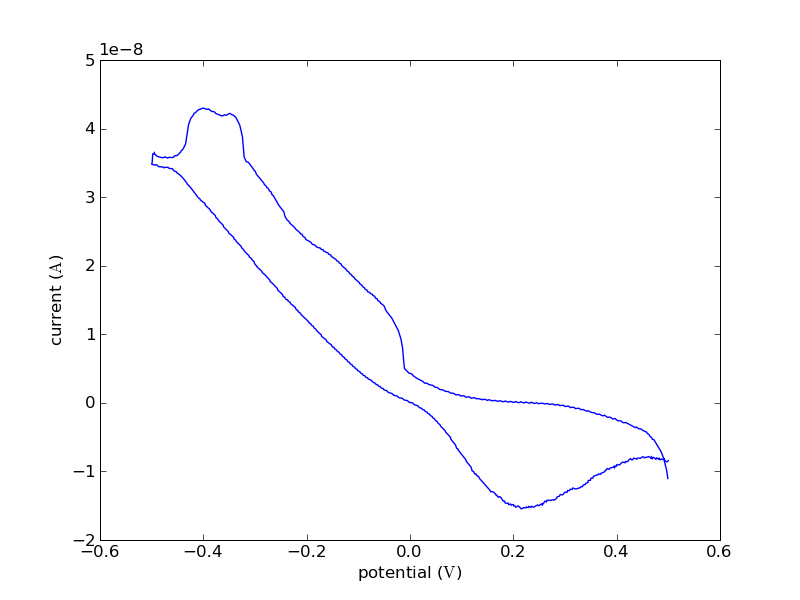
\includegraphics[width=0.5\linewidth]{figures/63.png}
\end{frame}

\begin{frame}{Differential Pulse Voltammetry}
	\begin{itemize}
		\item potential changes in increasing steps
		\item measures before and after change, returns difference
		\item removes charging current from output
		\item more accurate than CV
	\end{itemize}
	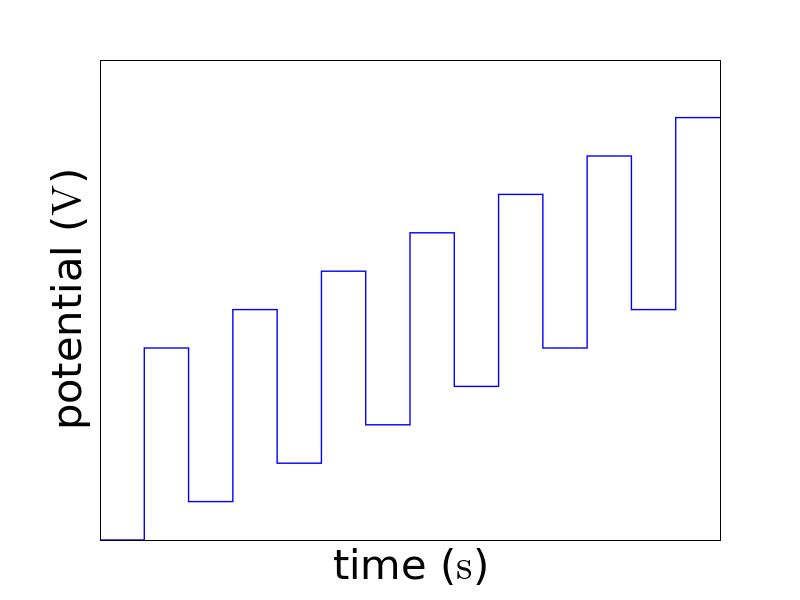
\includegraphics[width=0.5\linewidth]{figures/dpv.png}
	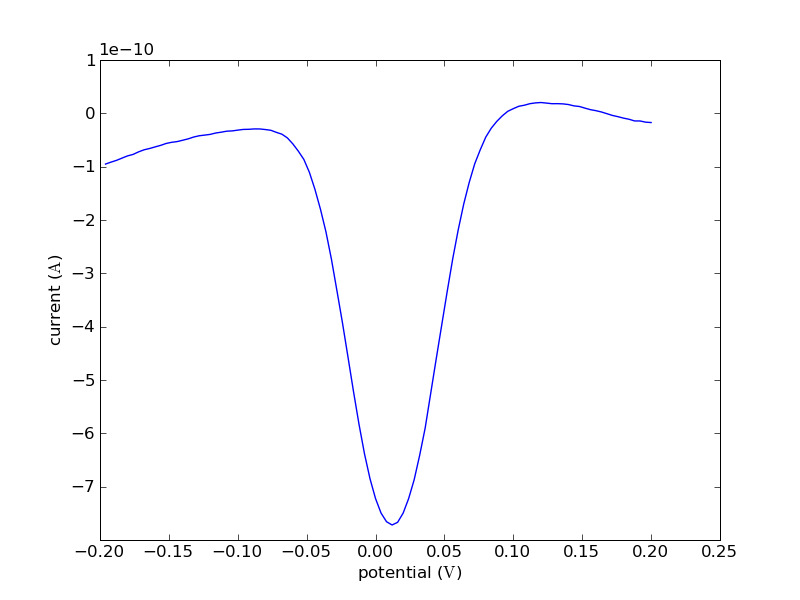
\includegraphics[width=0.5\linewidth]{figures/256.png}
\end{frame}

\subsection{Existing Approaches}
\begin{frame}{Existing Approaches}
	three fields of work:
	\begin{description}
		\item[smaller electrodes] for detection of lower concentrations and use in sensor arrays: in the last 20 years size has decreased from $250 \mu \mathrm{m}$ to $100 \mathrm{nm}$ \cite{shibuki1990emd, zhang2002nmn, bedioui1996cmm, zhang2002nse, kim2003img, wang2005mcn}
		\item[integrated potentiostats] for use on chip, no bulky additional instrument per sensor: various designs focusing on arrays, low currents, and uses in biosensors \cite{frey2003dip, murari2005ipn, stanacevic2007vpa, steffan2007scp}
		\item[electrode arrays] for detecting gradients: $2 \times 2$ to $4 \times 4$ arrays, all square or round (or unknown) shapes, no integrated potentiostats \cite{george2001fsp, naware2003dam, hafez2005eif, zhang2005eam}
	\end{description}
\end{frame}

\section{Chip Design and Characterization Results}
\subsection{Chip Design}
\begin{frame}{Chip Design}
	\begin{itemize}
		\item $5 \times 5$ array, 21 sensor sites
		\item each site has 4 working electrode (WE) areas
		\item each area has 1 or 2 WEs (for 3- and 4-electrode systems)
		\item sites have some similar configuration, but are all unique
		\item differing configurations allow testing of design hypotheses
	\end{itemize}
	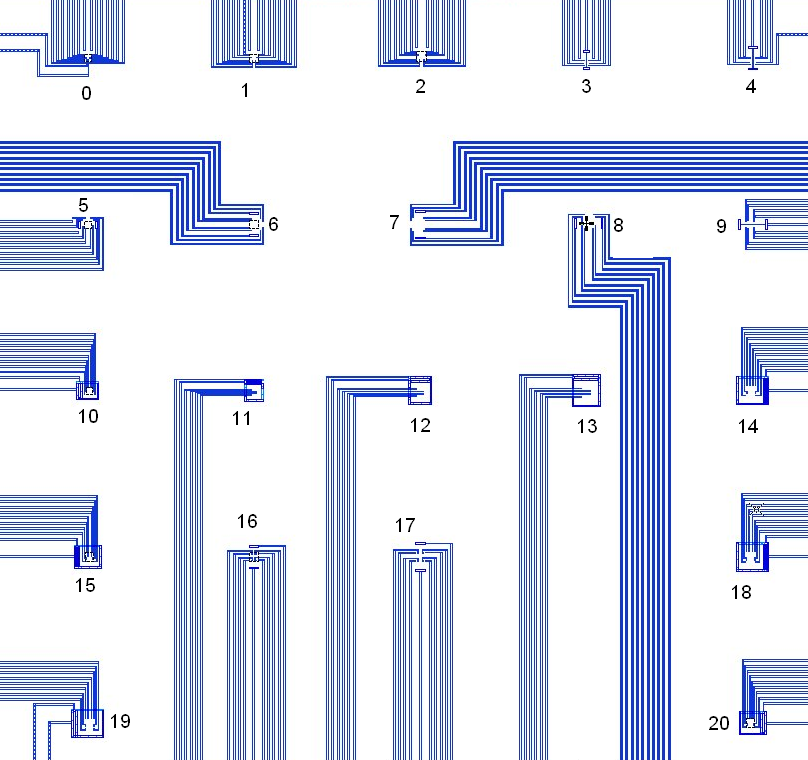
\includegraphics[width=0.5\linewidth]{figures/biosensorchip-sensors.png}
\end{frame}

\subsection{Working Electrodes}
\begin{frame}{Working Electrodes}
	\begin{itemize}
		\item 2 electrode systems: 3- and 4-electrode
		\item 4 WE types
			\begin{itemize}
				\item 3-electrode: all square shape
				\item 4-electrode, C shape
				\item 4-electrode, inverse C shape
				\item 4-electrode, F shape
			\end{itemize}
	\end{itemize}
	
\includegraphics[width=0.2\linewidth]{figures/4-C.png} \,
	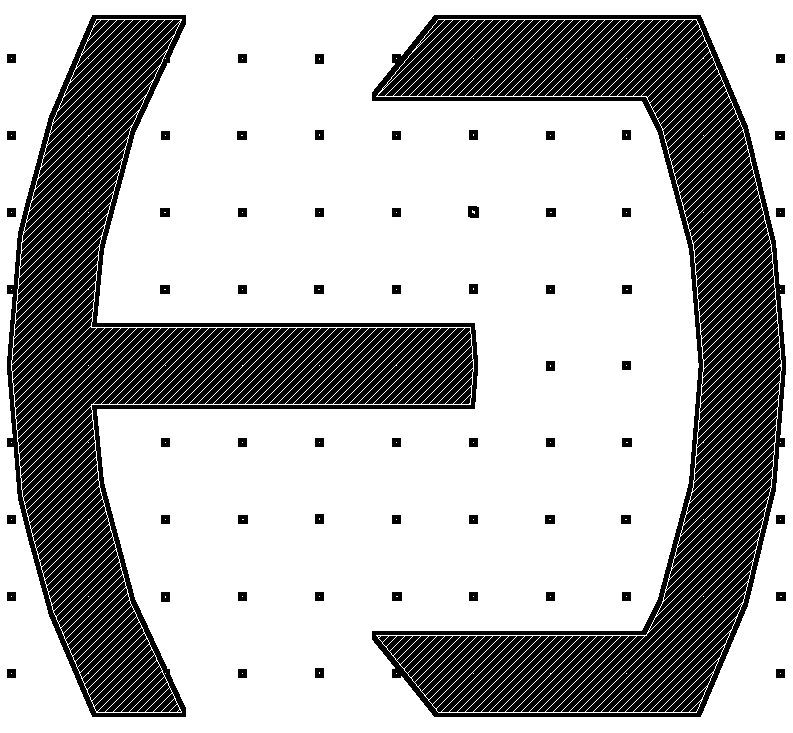
\includegraphics[width=0.2\linewidth]{figures/4-I.png} \,
	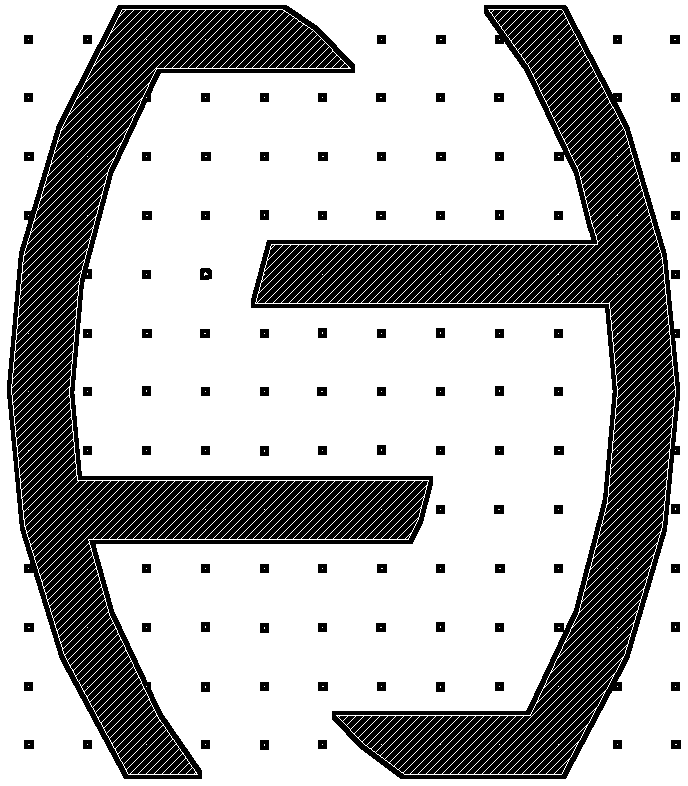
\includegraphics[width=0.2\linewidth]{figures/4-F.png}
\end{frame}

\subsection{Sites}
\begin{frame}{Sites (1 of 4 configurations)}
	\begin{block}{2 auxiliary}
		\begin{itemize}
			\item four electrodes, all same size and spacing
			\item 2 shorted auxiliary electrodes (AE) in diagonal corners
			\item always 3-electrode system
		\end{itemize}
	\end{block}
	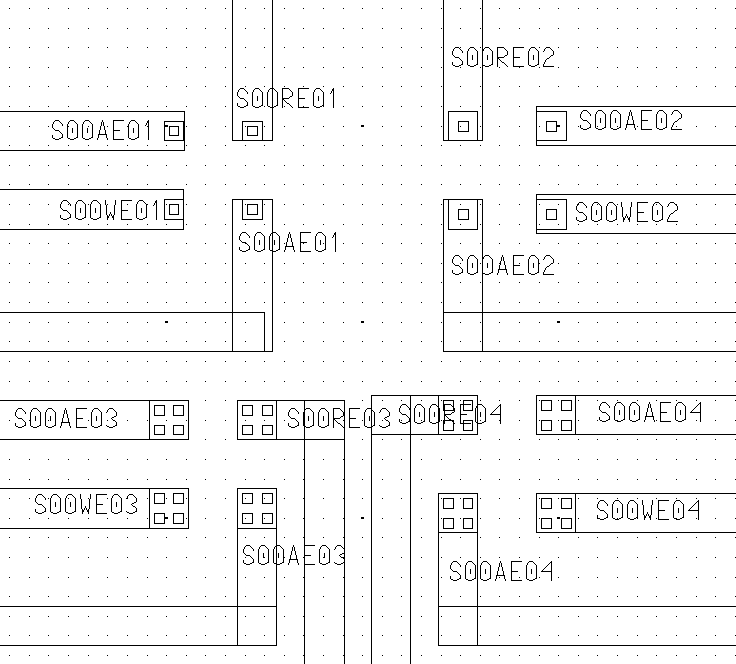
\includegraphics[width=0.5\linewidth]{figures/s00.png}
\end{frame}

\begin{frame}{Sites (2 of 4 configurations)}
	\begin{block}{common reference, top \& bottom}
		\begin{itemize}
			\item large reference electrode (RE) at top and bottom of site
			\item 4 pairs of WEs and AEs
			\item always 3-electrode system
		\end{itemize}
	\end{block}
	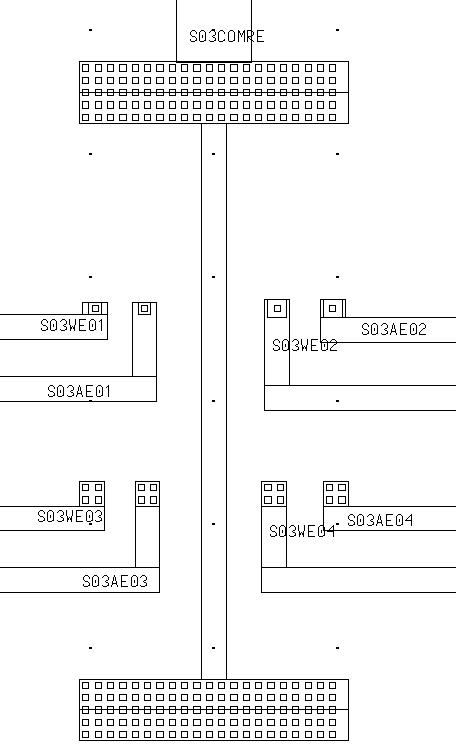
\includegraphics[width=0.3\linewidth]{figures/s03.png}
\end{frame}

\begin{frame}{Sites (3 of 4 configurations)}
	\begin{block}{common reference top, common auxiliary bottom}
		\begin{itemize}
			\item large reference electrode at top
			\item large auxiliary electrode at bottom
			\item 4 WE areas (either 3- or 4-electrode system)
		\end{itemize}
	\end{block}
	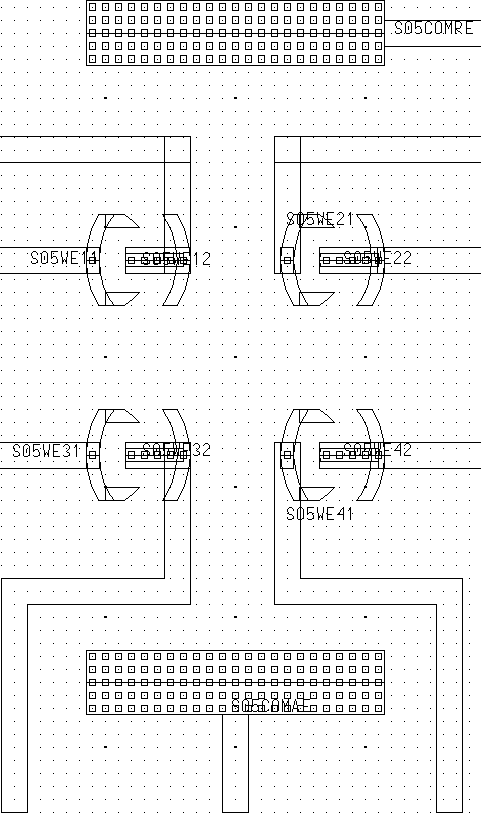
\includegraphics[width=0.3\linewidth]{figures/s05.png}
\end{frame}

\begin{frame}{Sites (4 of 4 configurations)}
	\begin{block}{common reference top, common auxiliary on 3 sides}
		\begin{itemize}
			\item large reference electrode at top
			\item large auxiliary electrode on top, left, bottom, and surrounding RE
			\item 4 WE areas (either 3- or 4-electrode system)
		\end{itemize}
	\end{block}
	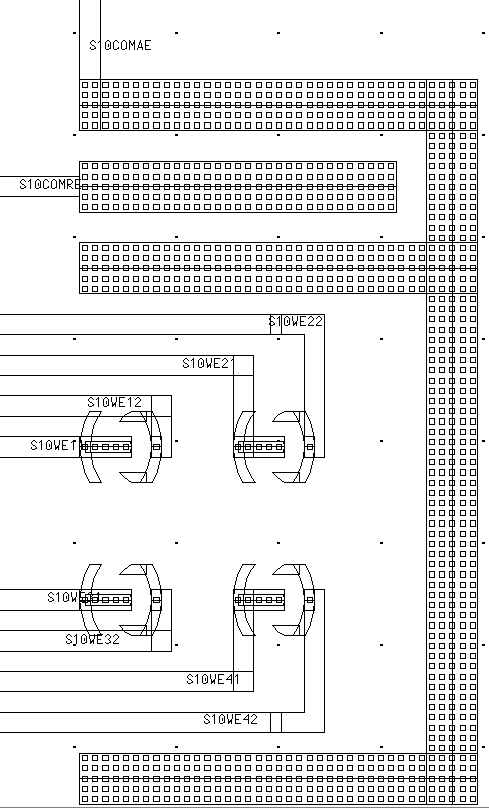
\includegraphics[width=0.3\linewidth]{figures/s10.png}
\end{frame}

\subsection{Experiment Setup}
\begin{frame}{Experiment Setup}
	\begin{itemize}
		\item create PDMS well, glue onto chip: holds solution
	\end{itemize}
	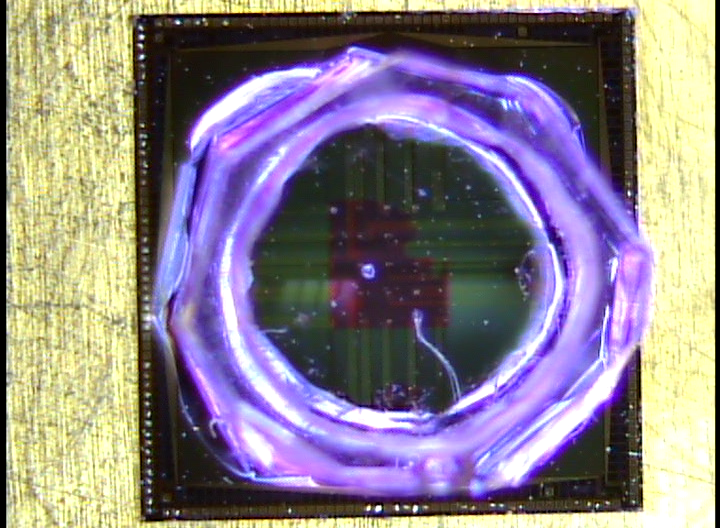
\includegraphics[width=\linewidth]{figures/chip-top.png}
\end{frame}

\begin{frame}{Experiment Setup}
	\begin{itemize}
		\item equipment: Faraday cage, CHI 660B potentiostat, probestation \& micromanipulators, PC
	\end{itemize}
	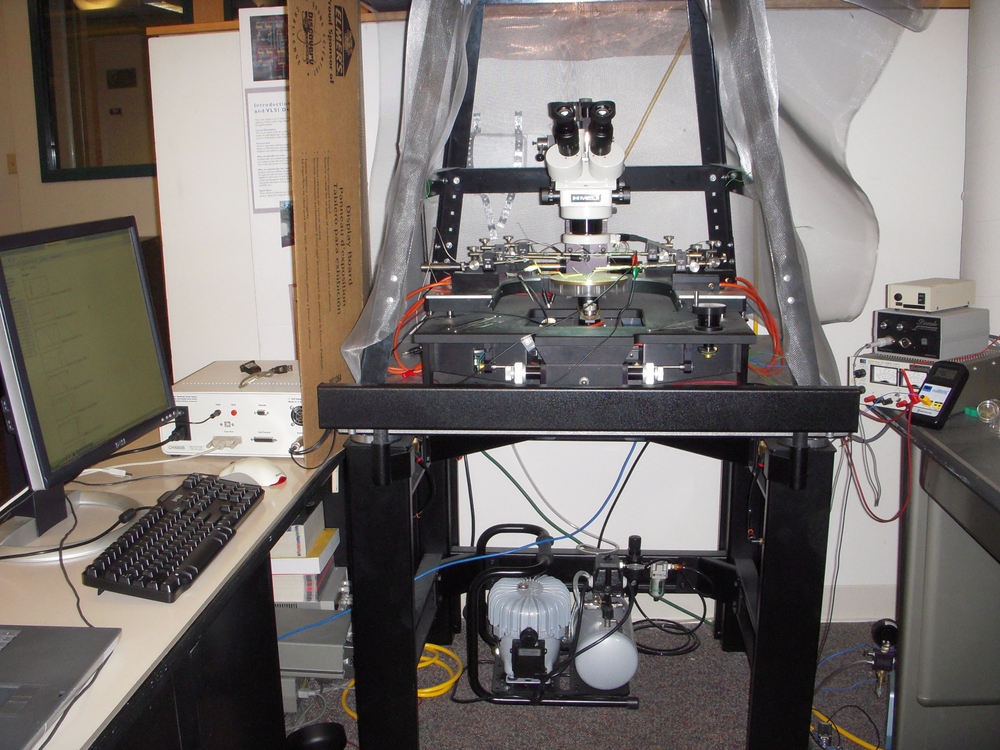
\includegraphics[width=0.95\linewidth]{figures/probestation.png}
\end{frame}

\begin{frame}{Experiment Setup}
	\begin{itemize}
		\item connect potentiostat leads to probe pins
		\item lower probe pins onto chip
	\end{itemize}
	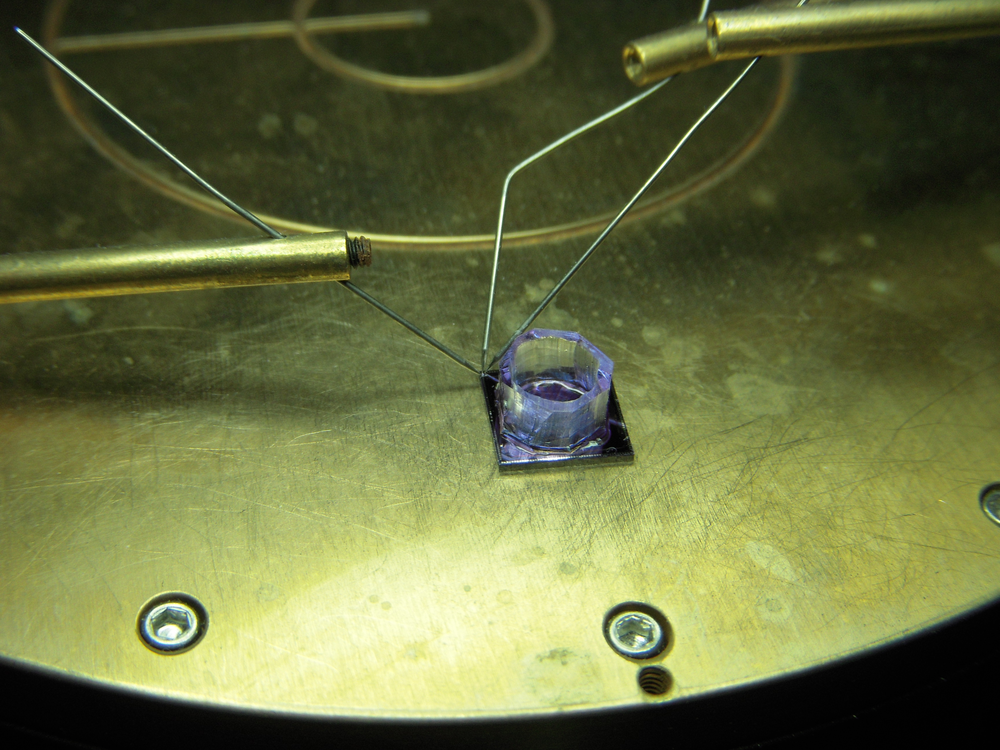
\includegraphics[width=0.5\linewidth]{figures/chippins.png}
	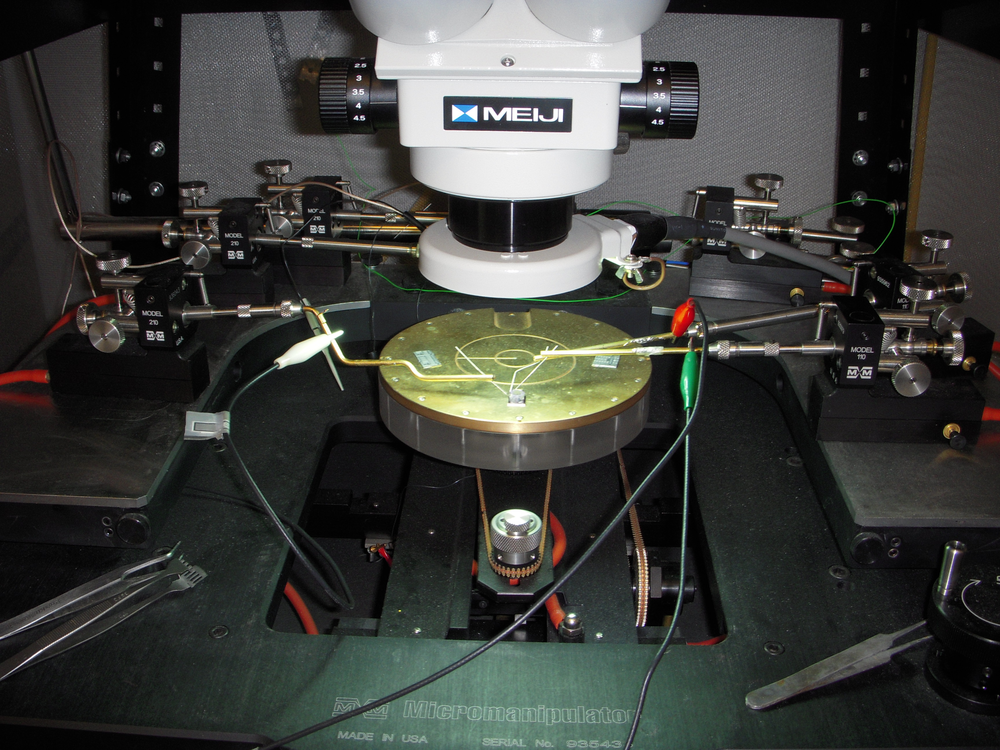
\includegraphics[width=0.5\linewidth]{figures/potentiostatleads.png}
\end{frame}

\subsection{Experiment Procedure}
\begin{frame}{Experiment Procedure}
	\begin{block}{all sites}
		test all 21 sites, 2 random WEs, 3 times each: 6 tests per site
	\end{block}
	\begin{block}{limit of detection}
		DPV on highest performing sites from above, decrease concentration until no results
	\end{block}
	\begin{block}{specific WEs}
		DPV on specific WEs to better test design hypotheses
	\end{block}
\end{frame}

\subsection{Experiment Results}
\begin{frame}{Output vs. Working Electrode Area}
	\textbf{hypothesis:} output proportional to WE area
	\begin{itemize}
		\item easily conclusive: design criteria
		\item however, lots of other variables, so maybe not that meaningful
	\end{itemize}
	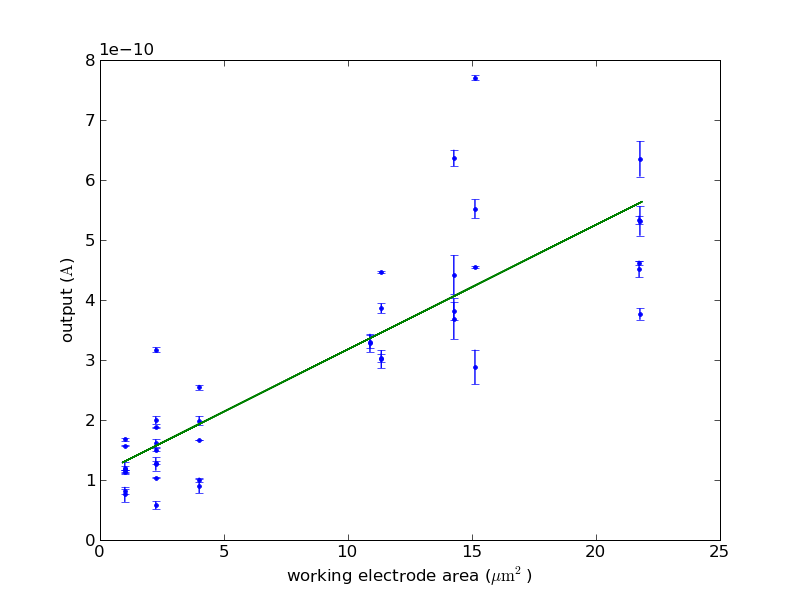
\includegraphics[width=0.8\linewidth]{figures/area_v_output.png}
\end{frame}

\begin{frame}{Output Density vs. Working Electrode Area}
	\textbf{hypothesis:} output density proportional to WE area
	\begin{itemize}
		\item general trend
		\item when split into 3- and 4-electrode systems, no conclusive data
	\end{itemize}
	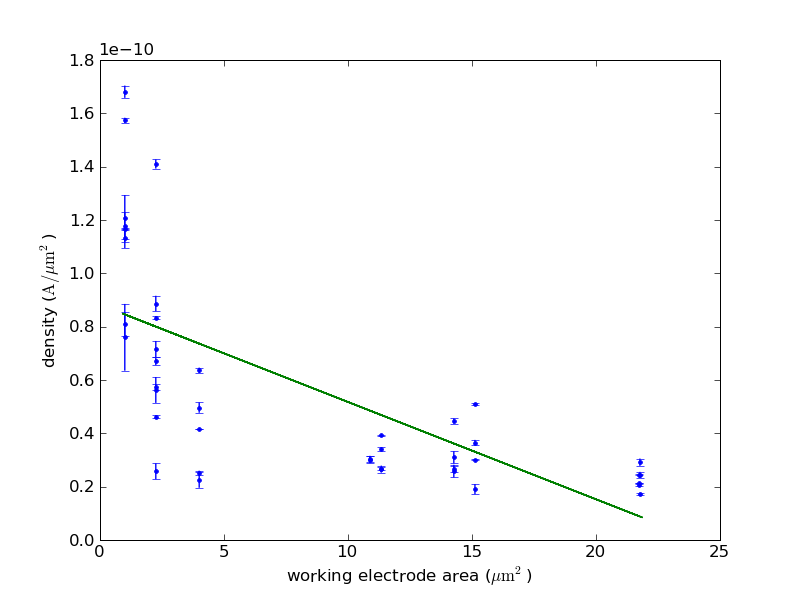
\includegraphics[width=0.8\linewidth]{figures/area_v_density.png}
\end{frame}

\begin{frame}{Output Density vs. Working Electrode Area}
	3-electrode systems
	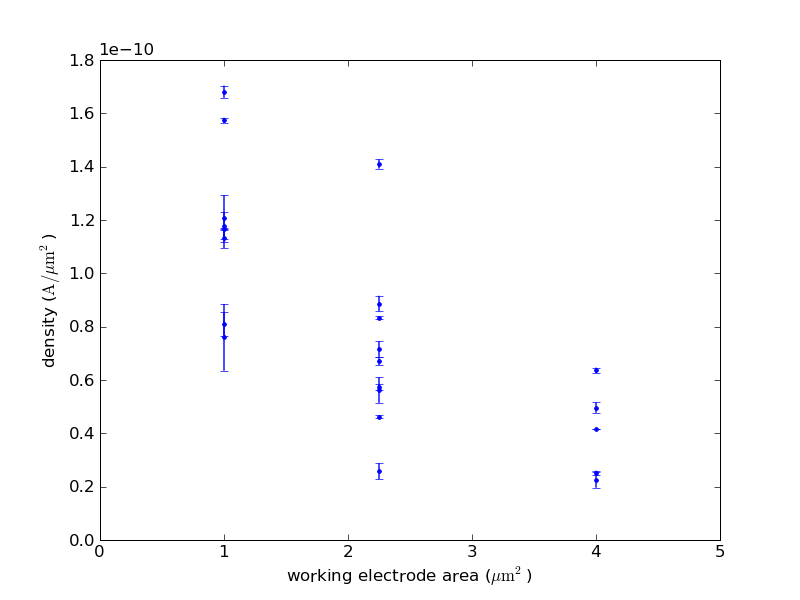
\includegraphics[width=0.8\linewidth]{figures/area_low_v_density.png}
\end{frame}

\begin{frame}{Output Density vs. Working Electrode Area}
	4-electrode systems
	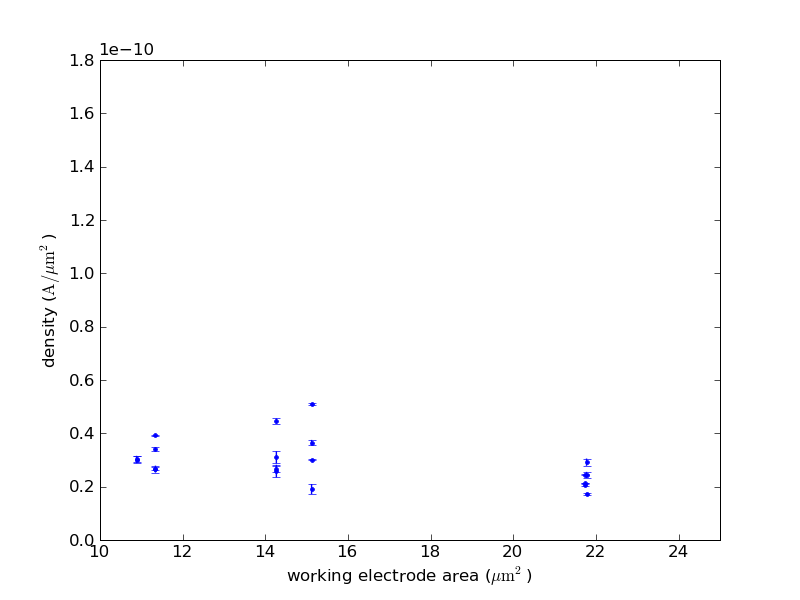
\includegraphics[width=0.8\linewidth]{figures/area_high_v_density.png}
\end{frame}

\begin{frame}{Ratio of Working to Auxiliary Electrode Areas}
	\textbf{hypothesis:} output proportional to ratio of WE to AE areas
	\begin{itemize}
		\item when ratio near unity, low output
		\item lower ratio (i.e., AE is large compared to WE) has larger outputs
		\item conclusive: design criteria
	\end{itemize}
	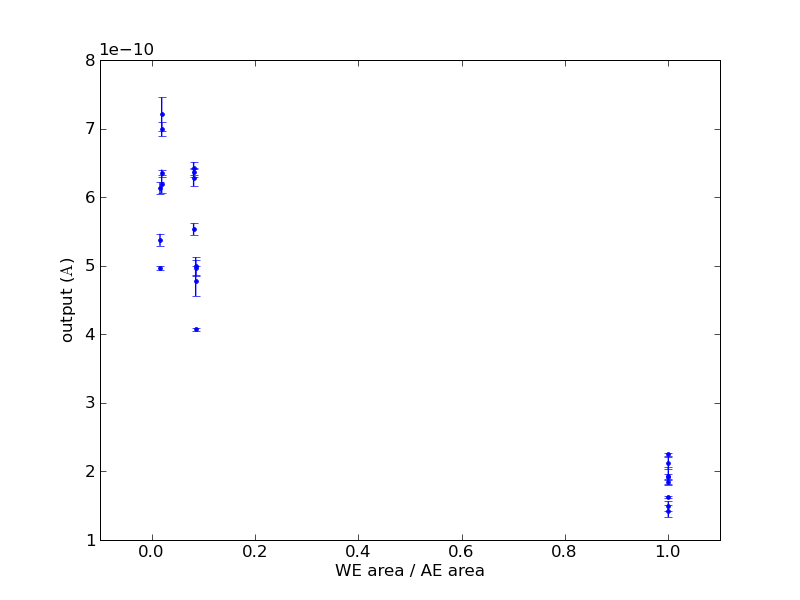
\includegraphics[width=0.8\linewidth]{figures/area_ratio_v_output.png}
\end{frame}

\begin{frame}{WE Perimeter over Area vs. Output Density}
	\textbf{hypothesis:} output density proportional to WE perimeter over area
	\begin{itemize}
		\item curve fits well, conclusive
		\item indicates most electron transfer occurs near electrode edge, which other work confirms
	\end{itemize}
	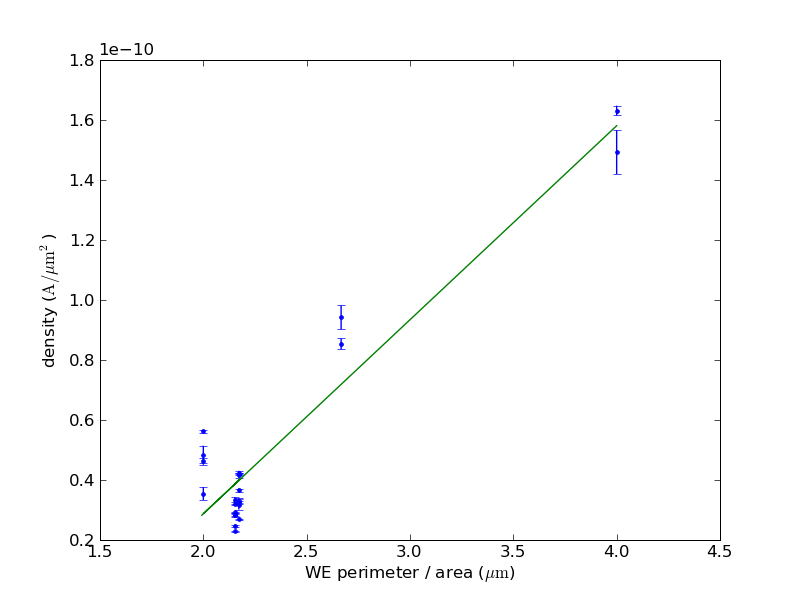
\includegraphics[width=0.8\linewidth]{figures/perim_area_v_density.png}
\end{frame}

\begin{frame}{Distance from Working to Auxiliary Electrode}
	\textbf{hypothesis:} output proportional to distance from WE to AE
	\begin{itemize}
		\item in general it appears distance plays a minor role: inconclusive
		\item perhaps distance matters when AE to WE area ratio is small
	\end{itemize}
	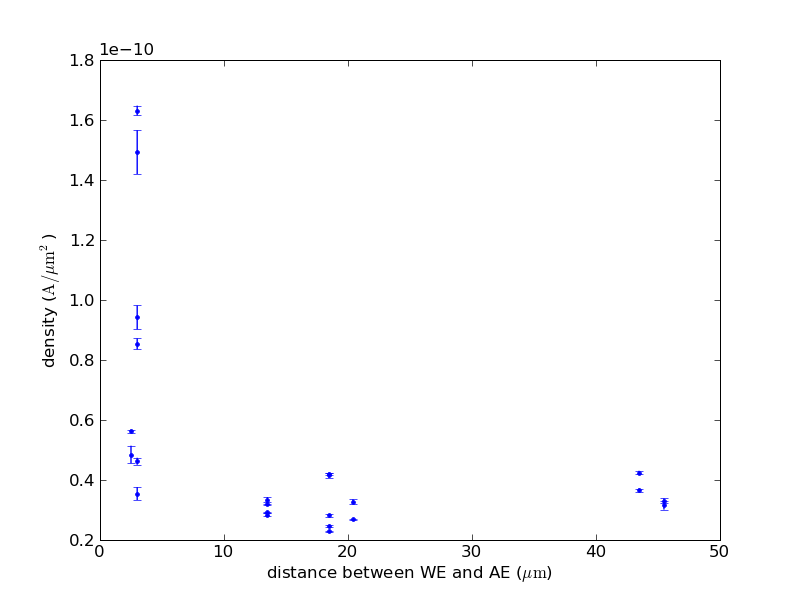
\includegraphics[width=0.8\linewidth]{figures/distance_v_density.png}
\end{frame}

\subsection{Limit of Detection}
\begin{frame}{Limit of Detection}
	\begin{itemize}
		\item tested sensors 17, 8 (best performers from all-sites test)
		\item 17 got down to $3 \mu \mathrm{M}$
		\item 8 got down to $10 \mu \mathrm{M}$
	\end{itemize}
	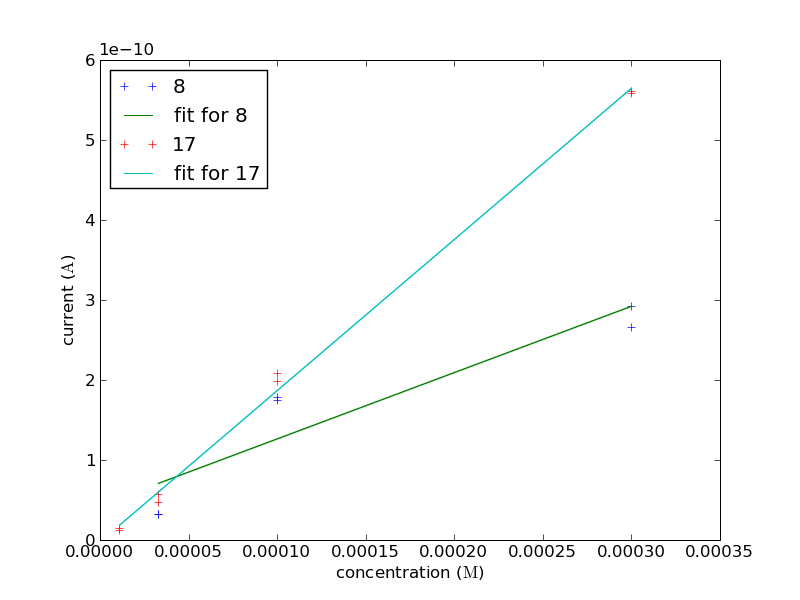
\includegraphics[width=0.8\linewidth]{figures/limit.png}
\end{frame}

\section{Slice Testing}
\begin{frame}{Slice Testing}
	\begin{itemize}
		\item this work is intended for living cells
		\item so we did some proof-of-concept tests with living cells
		\item mouse-ovary slices prepared by Biomedical Sciences at CSU
		\item $200 \mu \mathrm{m}$ thick from adult, female mice
		\item did our best to keep them alive through the end of testing
	\end{itemize}
\end{frame}

\subsection{Experiment Procedure}
\begin{frame}{Experiment Procedure}
	\begin{itemize}
		\item enclose in Faraday cage
		\item heat to $37\,^{\circ}\mathrm{C}$ with lamp
		\item run amperometry at $0.85 \mathrm{V}$ for 30 minutes
	\end{itemize}
	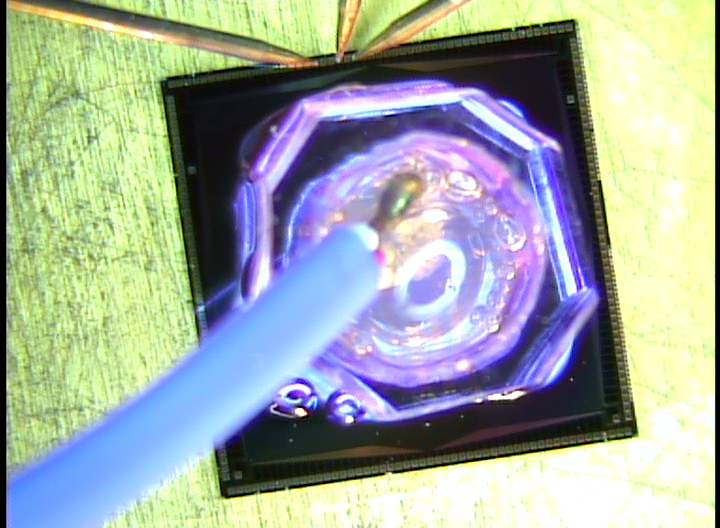
\includegraphics[width=0.8\linewidth]{figures/slice-top.png}
\end{frame}

\subsection{Experiment Results}
\begin{frame}{Experiment Results}
	\begin{itemize}
		\item outputs with current spikes and exponential return to baseline (consistent with release profile)
		\item comparable to previous work
		\item no quantitative data yet
		\item our electrodes are smaller, so we get smaller peaks and larger times
	\end{itemize}
	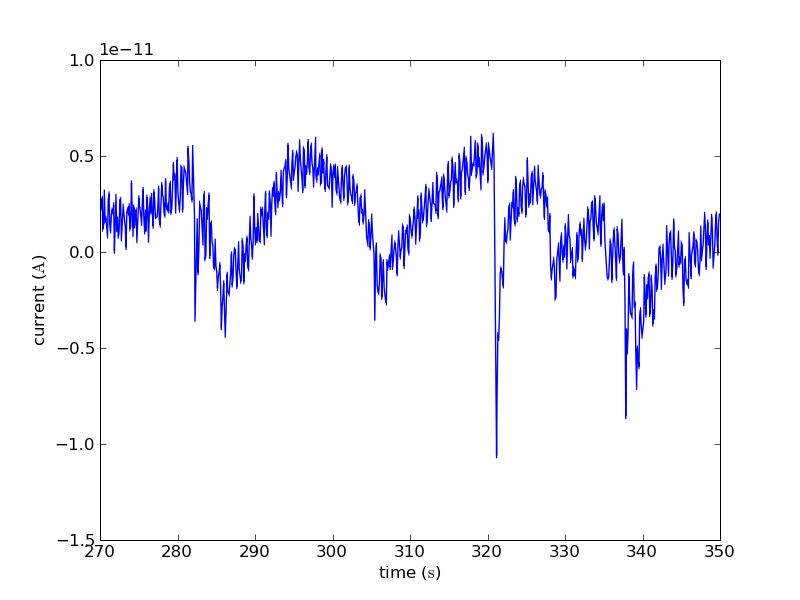
\includegraphics[width=0.5\linewidth]{figures/216.png}
	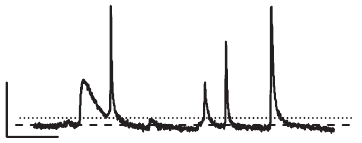
\includegraphics[width=0.5\linewidth]{figures/mosharok-pulse.png}
\end{frame}

\section{Conclusion}
\begin{frame}{Conclusion}
	\begin{itemize}
		\item built a working chip
		\item tested various design hypotheses
			\begin{description}
				\item[WE area] directly related to output
				\item[WE/AE ratio] inversely related to output
				\item[others] had inconclusive data \\ (shape, distance, configuration)
			\end{description}
		\item found limit of detection for some good sensors
		\item proof-of-concept work with ovary slices
	\end{itemize}
\end{frame}

\section{References}
\begin{frame}[allowframebreaks]{References}
	\bibliography{thesis}{}
	\bibliographystyle{ieeetr}
\end{frame}

\end{document}
